%atividades_psi.tex - Relatório parcial de atividades do projeto para a disciplina PSI2594

\documentclass[a4paper,12pt,font=plain,header=plain]{abnt}

\usepackage[brazil]{babel}
\usepackage[utf8]{inputenc}

\usepackage[alf]{abntcite}

\usepackage{tabularx}
\usepackage{verbatim}
\usepackage[final]{pdfpages}

\autor{Leandro Coletto Biazon\protect\\Nathalia Sautchuk Patrício}
\titulo{Febrace\textsuperscript{V}:\\Feira Brasileira Virtual de Ciências e
Engenharia}
\orientador[Orientadoras:\\]{Profª. Drª. Roseli de Deus Lopes\protect\\Profª. Drª. Selma
Shin Shimizu Melnikoff}
\instituicao{Escola Politécnica da Universidade de São Paulo\par Departamento de Engenharia de Sistema Eletrônicos}
\local{São Paulo}
\data{Maio de 2009}

\renewcommand{\ABNTchapterfont}{\bfseries\sffamily\fontseries{sbc}\selectfont}
\renewcommand{\ABNTsectionfont}{\bfseries\sffamily}

\begin{document}
\capa
%\folhaderosto

\renewenvironment{center}{}{}
\chapter*{PSI 2594 - PROJETO DE FORMATURA II}

  \begin{tabular}[|l|]{ |r|l| }
    \hline
      & Leandro Coletto Biazon, leandrobiazon@gmail.com (PSI) \\
    \hline
      & Nathalia S. Patrício, nathalia.sautchuk@gmail.com (PCS) \\
    \hline
      Orientadoras & Profª. Drª. Roseli de Deus Lopes, roseli@lsi.usp.br \\
    \hline
      & Profª. Drª. Selma S. S. Melnikoff, selma.melnikoff@poli.usp.br \\
    \hline
  \end{tabular} \\

  A1.a – Relatório Parcial de atividades (versão: 06/05/2009) \\

  \begin{tabularx}{0.9\linewidth}{ |r|r|X|r| }
    \hline
      \multicolumn{3}{|c|}{Campos a serem preenchidos pelo orientador, secretaria e comitê gestor} \\
    \hline
      Orientador & Data de Entrega &  \\
    \hline
      & De acordo &  \\
    \hline
      & &  \\
    \hline
      Secretaria & Data e hora de entrega &  \\
    \hline
      &  &  \\
    \hline
      Comitê Gestor &  &  \\
    \hline
      &  &  \\
    \hline
      \multicolumn{3}{|l|}{Comentários} \\
        \multicolumn{3}{|l|}{} \\
        \multicolumn{3}{|l|}{} \\
        \multicolumn{3}{|l|}{} \\
        \multicolumn{3}{|l|}{} \\
        \multicolumn{3}{|l|}{} \\
        \multicolumn{3}{|l|}{} \\
        \multicolumn{3}{|l|}{} \\
        \multicolumn{3}{|l|}{} \\
        \multicolumn{3}{|l|}{} \\
        \multicolumn{3}{|l|}{} \\
        \multicolumn{3}{|l|}{} \\
        \multicolumn{3}{|l|}{} \\
    \hline
  \end{tabularx}

\sumario

\chapter{Introdução}

  A Febrace (Feira Brasileira de Ciências e Engenharia), realizada todos os anos na Escola Politécnica da USP e organizada pelo Nate-LSI (Núcleo de Aprendizagem, Trabalho e Entretenimento do Laboratório de Sistemas Integráveis), é um projeto de ação contínua com o objetivo de estimular a criatividade, a reflexão, o aprofundamento e o raciocínio crítico nas atividades desenvolvidas por estudantes dos Ensinos Fundamental, Médio e Técnico, por meio da indução em realizar projetos investigativos em Ciências, Engenharia e suas aplicações\cite{lopes07}.

  Com o intuito de aumentar o alcance da Feira, levando-a por mais tempo a mais pessoas, e estimulando a criação de redes entre elas, o presente projeto propõe a criação de uma aplicação Web que possibilite o desenvolvimento e exposição dos projetos na Internet e que ofereça ferramentas que viabilizem maior interação entre os diversos envolvidos na Febrace (alunos participantes, professores orientadores, organizadores da Feira, avaliadores e público interessado).

  Assim, propõe-se:

  \begin{itemize}
    \item{
      Desenvolver e disponibilizar uma aplicação de código aberto que ofereça ferramentas para a exposição virtual de projetos de Ciência e Engenharia;
    }
    \item{
		Agregar à exposição virtual uma rede social que permita a interação entre os participantes da feira e que estes possam se ajudar com seus projetos e dirimir dúvidas de visitantes interessados em participar de suas futuras edições e
    }
    \item{
		Estudar e utilizar conceitos de usabilidade, acessibilidade e práticas de desenvolvimento web 2.0, aplicando metódos ágeis de desenvolvimento de \textit{software}.
    }
  \end{itemize}

  \section{Objetivo}
    O projeto tem como objetivo desenvolver uma rede social focada em desenvolvimento e exposição de projetos de ciências e engenharia. Dentre os conceitos de engenharia de \textit{software} a serem aplicados no projeto, destacam-se a temática de usabilidade e acessibilidade, metódos ágeis de desenvolvimento de \textit{software} e práticas de desenvolvimento web.

\chapter{Programação extrema}
  A programação extrema (\textit{eXtreme Programming} ou XP) é um método leve para que equipes pequenas ou médias desenvolvam \textit{software} em face a requisitos vagos ou que mudem constantemente\cite{beck04}. Pela definição de seu autor, Kent Beck, o XP é leve porque é focado na realização das tarefas que criem valor para o cliente. Seu principal objetivo é o desenvolvimento de \textit{software} com qualidade, por meio de um estilo de desenvolvimento focado nas melhores práticas de programação, comunicação clara e trabalho em equipe.

  Como outras metodologias ágeis, o XP se opõe a diversas premissas assumidas pelas metodologias tradicionais de engenharia de \textit{software}. Uma dessas premissas é que é possível prever todos os passos necessários para o desenvolvimento de um sistema, pelo detalhado levantamento de características do problema a ser resolvido e da solução a ser desenvolvida. O XP assume a presença constante das mudanças durante o processo de desenvolvimento, e propõe uma série de práticas para lidar com elas.

  A programação extrema é descrita por meio de seus valores, princípios e práticas. As práticas são uma série de técnicas a serem aplicadas no dia-a-dia de trabalho da equipe. Os valores são a noção do que é certo e do que é errado no relacionamento da equipe com o trabalho e entre si. Os valores são o que fundamentam as práticas. Porém os valores do XP são universais e independem do contexto do desenvolvimento de \textit{software}, estando assim muito distante das práticas. A ponte entre os valores e as práticas são os princípios, que trazem orientações para um contexto específico.

  \section{Valores}
    O primeiro dos valores do XP é a \textbf{Comunicação}, por pressupor que a maioria dos problemas de um projeto ocorrem por dificuldades nesse aspecto. A comunicação constante e eficaz entre os membros da equipe permeia todo processo de desenvolvimento, e é ressaltado em diversas das práticas do XP.

    Outro princípio é a \textbf{Simplicidade}, que leva a equipe a buscar sempre as soluções mais simples a um dado problema, sem tentar otimizações precoces ou a a tentativa de resolução de um problema futuro.

    Como não há uma direção pré-definida a ser seguida, a equipe de XP precisa constantemente saber onde se encontra para poder determinar seus próximos passos. O valor que orienta a equipe à rápida resposta sobre as ações realizadas é o \textbf{Feedback}.

    \textbf{Coragem} é a ação efetiva frente à insegurança, para a tomada de decisões necessárias ao projeto.

    O último valor é o \textbf{Respeito}. Os membros da equipe devem se importar uns com os outros e com as ações realizadas.

  \section{Princípios}

    Os princípios definidos na segunda edição do livro \textit{Extreme Programming Explained}\cite{beck04} são as seguintes:

    \begin{description}
      \item[Humanidade]
	      O \textit{software} é desenvolvido por pessoas. As necessidades pessoais dos membros da equipe devem ser levadas em consideração no processo de desenvolvimento.
      \item[Economia]
        A produção de \textit{software} não está à parte do processo econômico, e seus aspectos devem ser considerados.
      \item[Benefício mútuo]
        Qualquer atividade deve beneficiar todas as pessoas envolvidas (desenvolvedores e clientes). Decisões emergenciais, que custem a uma pessoa, representam uma perda ao projeto como um todo.
      \item[Auto semelhança]
        A estrutura de uma solução deve ser utilizada em outros contextos, mesmo que em diferentes escalas.
      \item[Aperfeiçoamento]
        Deve-se sempre buscar a realização do melhor trabalho possível, hoje.
      \item[Diversidade]
        As equipes devem ser formadas por pessoas com diferentes perfis. Os conflitos que possam surgir dessa escolha são compensados pelo benefício das múltiplas visões sobre um problema.
      \item[Reflexão]
        Não é suficiente realizar tarefas, é necessário constantemente revisitar o trabalho feito e refletir sobre as decisões tomadas, analisando as razões dos sucessos e das falhas.
      \item[Fluxo]
        O fluxo é a realização simultânea de várias etapas do processo de desenvolvimento, ao invés de separar as fases e trabalhá-las isoladamente.
      \item[Oportunidade]
        Problemas devem ser vistos como oportunidades de mudança.
      \item[Redundância]
        Normalmente vista como desperdício, a redundância é o melhor caminho para lidar com as falhas, e deve ser empregada em diversos contextos (múltipla resolução de um problema, programação pareada, etc.).
      \item[Falha]
        Quando não se sabe a maneira de resolver um problema, deve-se implementar uma alternativa que falhe, e aprender com ela. As falhas não são um desperdício, e sim conhecimento.
      \item[Qualidade]
        Qualidade não deve ser vista como uma variável de controle, negociável, e deve ser sempre buscada.
      \item[Pequenos passos]
        Ao dar grandes passos, leva-se muito tempo para realizá-los e, caso tenham sido dados na direção errada, é mais difícil voltar atrás. Agindo dessa maneira, é frequente o temor da necessidade de mudanças. Pequenos passos são uma postura mais adequada em processos complexos.
      \item[Aceitação de responsabilidade]
        A responsabilidade não deve ser designadas, devem ser aceitas.
    \end{description}

  \section{Práticas}
    As práticas são o que se vê no dia-a-dia de uma equipe de XP. Elas não devem ser adotadas, entretanto, desvinculadas dos valores e princípios mencionados anteriormente, sob o risco de se tornarem vazias. Na primeira edição de seu livro principal, Beck definiu 12 práticas, e mencionou que elas deveriam ser adotadas todas simultaneamente. Na edição mais recente, o autor muda a abordagem, dizendo que a adoção das práticas pode ser feita parcialmente, conforme as necessidades e experiências da equipe. Também nessa edição as práticas, agora 24, são divididas em dois grupos, primárias e corolárias. As práticas primárias são aquelas que devem ser tentadas primeiro pelas equipes, na sequência que se mostrar adequada. Já as práticas corolárias são mais difíceis de serem aplicadas, e requerem a experiência anterior com as práticas primárias. Nesse projeto serão trabalhadas, principalmente, as práticas primárias, descritas a seguir.

	\begin{description}
		\item[Sentar Junto]
		O ambiente de trabalho da equipe deve ser compartilhado. Há sim a necessidade de espaços privados, mas a equipe deve trabalhar junta, fisicamente, a maior parte possível do tempo.
		\item[Time completo]
		As equipes de XP devem ter pessoas com diversas habilidades diferentes, que atendam todas as necessidades de um projeto
		\item[Área de trabalho informativa]
		Uma pessoa que entre no espaço de uma equipe deve poder, num curto espaço de tempo, ter noção do estado em que se encontra o projeto em desenvolvimento. O ambiente deve propiciar também espaços coletivos para a programação e espaços individuais para a privacidade. Nas paredes, é interessante manter gráficos grandes, bem como outras informações pertinentes sobre o estado do projeto e da equipe.
		\item[Trabalho energizado]
		Só as horas produtivas devem ser trabalhadas. Trabalhar mais do que um limite apenas reduz o rendimento de um programador no resto da semana.
		\item[Programação pareada]
		Todo o código, exceto o escrito como experimentação, deve ser escrito com duas pessoas no mesmo computador.
		\item[Histórias]
		O planejamento deve ser realizado usando uma descrição de funcionalidades compreensível pelo cliente, por meio de cartões de história. Tão logo uma história é escrita, deve-se estimar o esforço necessário para implementá-la.
		\item[Ciclo semanal]
		O trabalho deve ser planejado uma semana por vez, e na reunião no início dessa semana a) reflita sobre a semana anterior, b) escolha um conjunto de histórias ainda não implementadas e c) quebre as histórias em tarefas.
		\item[Ciclo trimestral]
		Planejamentos de nível mais alto devem ser realizados trimestralmente. A cada trimestre devem ser levantados quais são os gargalos que impedem o time de prosseguir, e determinado o tema do próximo trimestre.
		\item[Folga]
		Tarefas menos importantes devem ser incluídas no planejamento, para que possam ser descartadas em caso de atrasos. A folga, seja ela com relação a tarefas, orçamento ou horas trabalhadas deve ser considerada em um projeto.
		\item[\textit{Build} em 10 minutos]
		A compilação e realização dos testes automáticos de um projeto devem ser realizados em 10 minutos.
		\item[Integração contínua]
		O código recém escrito e os testes a ele associados devem ser integrados constantemente no corpo de código do projeto, no máximo a cada 2 horas.
		\item[Desenvolvimento dirigido por testes]
		Testes automáticos devem ser escritos antes de uma parte do sistema ser modificada.
		\item[Design incremental]
		O design de um sistema deve ser trabalhado diariamente, levando-se em consideração o melhor a ser feito naquele momento.
	\end{description}

	\section{Programação extrema no contexto acadêmico}
	Uma das metas do projeto é testar a validade de um conjunto de práticas propostas pela programação extrema, e experimentar sua consistência quando aplicada no contexto acadêmico. Objetiva-se também documentar essa experiência de forma que outros alunos que também queiram trabalhar com essas metodologias em seus projetos na universidade tenham um relato no qual se basear, com possíveis heurísticas e adaptações que se fizeram necessárias nesse caso em particular.

	Tendo isso em vista, realizou-se uma pesquisa por artigos que descrevessem experiências semelhantes de aplicação de metodologias ágeis na graduação. Foram encontrados diversos relatos dessa natureza, muitos deles descrevendo a utilização dessas metodologias em projetos de conclusão de curso.

	\citeonline{schneider03} avaliam a aplicação da programação extrema no contexto acadêmico, avaliando num plano teórico as práticas do XP e sua conformidade com o currículo de Engenharia de Computação do instituto onde lecionam. \citeonline{noble04} e \citeonline{keefe04} ministraram disciplinas de projetos de conclusão de curso onde o XP foi apresentado com uma das possíveis metodologias a serem escolhidas pelos alunos, e relatam nos artigos suas experiências.

	No artigo de \citeauthoronline{schneider03}, o XP é descartado como uma metodologia compatível com os objetivos da universidade. Cabe observar que os autores não se baseiam em nenhuma experiência real. \citeauthoronline{noble04} e \citeauthoronline{keefe04}, pelo contrário, consideram as experiências em seus cursos bem sucedidas, ressaltando a qualidade presente nos projetos desenvolvidos e a melhor interação entre os membros da equipe.

	Apesar das relatos positivos envolvendo a aplicação desse método ágil no contexto acadêmico, uma série de adaptações foi necessária para adequá-la aos cursos. As principais dificuldades citadas na utilização dessa metodologia na universidade foram:

	\subsection{Área de trabalho compartilhada}
		Os laboratórios das universidades, assim como suas salas de aula, não foram projetados para possibilitar a colaboração entre seus alunos. Um espaço de trabalho coletivo e informativo, preconizado pelo XP, não está a disposição das equipes.

	\subsection{Disponibilidade de tempo}
		Por ser dirigido ao ambiente corporativo, o XP define uma semana de trabalho de 40 horas, de impossível reprodução num curso universitário.

	\subsection{Presença do cliente}
		A presença do cliente na equipe de XP, incomum mesmo em empresas, é ainda mais difícil na universidade.

	\subsection{Necessidade de \textit{coaching}}
		Normalmente as equipes não tem nenhuma experiência anterior com o XP, e a presença do coach é importante para a aprendizagem da metodologia.

	\subsection{Testes}
		As experiências relatam dificuldades na utilização de testes automáticos, seja por problemas culturais (como a pouca importância dada a esse tópico no restante do currículo), seja por aspectos técnicos.

	\subsection{Formas de avaliação}
		Grande parte das avaliações realizadas nas disciplinas de projeto de conclusão de curso é baseada na documentação levantada por etapas das metodologias tradicionais. A criação desses documentos não é parte do processo das metodologias ágeis e outros critérios de avaliação apropriados a esse contexto foram necessários nas experiências apresentadas.

	\section{Programação extrema na Febrace\textsuperscript{V}}
	Em consequência dos motivos apresentados na sessão anterior, uma série de adaptações foi necessária para adequar a utilização da programação extrema ao contexto do projeto. As principais são descritas a seguir.

	\subsection{Espaço de trabalho compartilhado virtual}
		Não será possível dispor de um espaço de trabalho fixo para a realização das atividades referentes ao projeto. Na tentativa de suprir essa necessidade, será feito uso de um conjunto de ferramentas de trabalho colaborativo pela Internet, entre elas um "quadro branco" virtual e uma ferramenta de acompanhamento de \textit{bugs}. Mais detalhes sobre algumas dessas ferramentas são apresentados na sessão \textbf{Tecnologias utilizadas}.

	\subsection{Semana de 10 horas}
		Espera-se que a semana de trabalho da equipe seja de 10 horas.

	\subsection{Iterações}
		O tempo escolhido para cada iteração foi de três semanas. Assim, serão realizadas quatro iterações até o fim do primeiro semestre.

	\subsection{Cliente}
		O papel do cliente foi designado a um pesquisador do NATE-LSI que participa da organização da Febrace. Ele não estará sempre presente durante o desenvolvimento do projeto, mas serão realizadas reuniões semanais com ele.

	\subsection{Programação pareada}
		Todo o código de produção será escrito em sessões de programação pareada.

	\subsection{Retrospectivas}
		A restropectiva é uma reunião periódica na qual é avaliado o período anterior do projeto (entre aquela retrospectiva e a anterior). Nessa reunião participa toda a equipe de desenvolvimento e nela procura-se levantar coisas que deram certo naquele período, coisas que precisam ser melhoradas e idéias (desde do projeto em si até coisas referentes ao ambiente de trabalho) que possam ter surgidos durante esse período. Não há um tempo pré-determinado entre retrospectivas, mas para equipes que trabalham em período integral juntas é aconselhável que sejam quinzenais, enquanto não é ideal que demorem mais que um mês para ocorrer. Como uma adaptação ao processo, foi decidido que no caso do projeto em questão essas restrospectivas ocorrerão mensalmente e com base nelas serão escritos os documentos de acompanhamento a serem entregues na disciplina.

\chapter{Levantamento do perfil dos usuários}
  Um dos objetivos do projeto é o estudo dos conceitos de usabilidade, aplicando-os no desenvolvimento da Febrace\textsuperscript{V}. Para se fazer um estudo de usabilidade verificou-se como necessário um levantamento prévio com possíveis usuários do sistema para verificar o seu perfil de uso e suas reais necessidades em relação a uma nova ferramenta computacional. Como a sétima edição da FEBRACE ocorreria no primeiro semestre, viu-se a possibilidade de fazer esse levantamento com os participantes da feira que são potenciais usuários da rede social. O método escolhido para fazer esse levantamento foi através de questionário aplicados a finalistas, orientadores e visitantes durante a feira.

  \section{Elaboração do questionário de perfil de uso}
    O questionário proposto pelos integrantes do projeto foi avalidado pela equipe da FEBRACE e por outras pessoas com experiência em levantamento de dados com usuários, e a partir de suas sugestões foram feitos melhoramentos no questionário de perfil de uso de Internet dos participantes da feira.

    O questionário final, apresentado no Apêndice 1, apresenta três partes. A primeira tem por objetivo colher alguns dados demográficos, como idade, local de residência e escolaridade. Na segunda parte há perguntas que procuram identificar o perfil de uso da internet do usuário (de onde e com qual frequência ocorre o acesso, quais serviços são utilizados, etc.). O objetivo da terceira parte é saber a opinião dos usuários sobre sua atual experiência com os serviços web da FEBRACE e sobre seu interesse nas possíveis ferramentas oferecidas pela Febrace\textsuperscript{v}.

  \section{Aplicação do questionário}
    A FEBRACE ocorreu nos dias 17, 18 e 19 de março e durante esse período foram aplicados questionários para alunos e professores participantes, além de visitantes da feira. Foram respondidos 520 questionários. Até o presento momento foram compilados 136 questionários, 26\% do total.

  \section{Automação do processamento de dados coletados}
    O método escolhido para a aplicação do questionário foi em papel. Porém, com o objetivo de facilitar tanto a inserção de dados no computador quanto a compilação desses dados decidiu-se pelo uso de alguma ferramenta online. O questionário começou a ser transposto para o SurveyMonkey, porém a conta gratuita desse serviço é restrita a dez perguntas no questinário e cem questionários respondidos, limitações que tornam o serviço aquém das necessidades.

    Mais adequada é a ferramenta LimeSurvey, uma \textit{webapp} de código aberto que foi instalada e configurada localmente. Com ela os dados de cada questionário podem ser inseridos de forma mais rápida e prática e, pelo fato de estar \textit{online}, o trabalho poder ser mais facilmente entre os membros do grupo. Além disso, a ferramenta gera diversas estatísticas e desenha os respectivos gráficos.

\chapter{Levantamento de Histórias}

  O planejamento em XP feito com Histórias escritas em pequenos cartões. Cada cartão é escrito pelo cliente e deve descrever uma unidade de funcionalidade, que geralmente representa um requisito funcional desejado\cite{sato07}.

  Como uma forma de especificar o sistema a ser desenvolvido durante o projeto de formatura optou-se por descrever as histórias levantadas. As histórias foram escritas em conjunto com o cliente.

	\begin{enumerate}
	 \item Convite a ex-participantes \\
		Quero, como administrador do sistema, que seja enviado automaticamente um convite para participação na rede social para todos os participantes de edições anteriores da FEBRACE (cadastrados em um banco de dados legado). Caso o ex-participante crie seu perfil na rede social, o projeto dele deve ser criado automaticamente e associado a ele.
	 \item Autenticação no sistema \\
		Quero, como usuário, acessar a página inicial com meu e-mail e senha para me autenticar no sistema. Caso esqueça minha senha, quero informar o sistema e pedir que envie uma nova senha para meu e-mail. Se não for um usuário registrado, quero que me seja apresentada a tela de cadastro de novo usuário.
	 \item Cadastro de Usuário \\
		Quero poder criar um perfil no sistema através de cadastro no sistema fornecendo um e-mail válido e uma senha para o acesso.
	 \item Edição de Perfil \\
		Quero, como usuário registrado, poder editar a página de meu perfil pessoal, alterando, inserindo e excluindo os dados lá presentes, e escolhendo quais usuários podem ter acesso a determinadas informações minhas.
	 \item Visualização de Perfil \\
		Quero, como usuário, poder visualizar meu perfil e de meus amigos, bem como, via sistema de busca, visualizar os perfis de quem o permita a qualquer usuário.
	 \item Cancelamento de Cadastro \\
		Quero, como usuário, poder quando assim desejar cancelar meu cadastro do sistema.
	 \item Visualização de Projeto \\
		Quero, como usuário, ver as informações de cada projeto, como seu nome e resumo, sua área do conhecimento, participantes e demais informações relevantes.
	 \item Visualização de Participantes de um projeto \\
		Quero, como usuário, ver na página de um projeto quais são seus participantes, e ter acesso a seus perfis. Gostaria de saber também qual seu papel na Feira (estudante, orientador, etc.) e a instituição a qual pertence.
	 \item Visualização de Vídeo de um projeto \\
		Quero, como usuário, poder ver na página de um projeto, quando disponível, seu vídeo oficial, feito na própria FEBRACE, hospedado em um site dedicado como a IPTV-USP ou o Youtube.
	 \item Visualização de prêmios de um projeto \\
		Quero, como usuário, saber quais prêmios foram ganhos por algum projeto na edição da feira em que participou. Quero também poder acessar mais informações sobre esses prêmios.
	 \item Edição dos Conteúdos de um projeto \\
		Quero, como participante de um projeto, poder inserir novas informações em sua página, como textos (relatório, diário de bordo, etc.), fotos e vídeos relacionados com ele, entre outros. Quero também poder editar esses conteúdos por mim adicionados, modificando-os ou apagando-os.
	 \item Edição de Diário de Bordo de um projeto \\
		Quero que cada projeto tenha a ele associado uma ferramenta que permita a criação de um diário de bordo online, com o formato de \textit{weblog}.
	 \item Adicionar amigos \\
		Quero, como usuário, escolher quais outros usuários são meus amigos, dando a eles permissão de me escrever mensagens, entre outras operações.
	 \item Adicionar projetos prediletos \\
		Quero, como usuário, fazer uma lista de projetos que mais me chamaram atenção na feira. Quero poder fazer um comentário que justifique minha indicação, se assim o desejar.
	 \item Postar em fórum \\
		Quero, como usuário, ter um espaço que permita postar perguntas que outros usuários possam responder, avisos, notícias e quaisquer outro tipo de texto relacionado.
	 \item Comentar em caixas de comentários \\
		Quero, como usuário, poder deixar comentários nas diversas páginas da rede social, como projetos, artigos e diários de bordo. Caso eu tenha feito o comentário estando logado, ele deve ser identificado e deve haver um link para meu perfil nele. Comentários de visitantes podem ou não ser aceitos a critério de quem administra o conteúdo comentado.
	 \item Enviar mensagens a outros usuários \\
		Quero, como usuário, enviar mensagens privadas de texto a outros usuários e receber mensagens enviadas por ele. Quero também poder escolher quais usuários podem ou não me escrever.
	 \item Buscar conteúdos do sistema \\
		Quero, como usuário, ter acesso a  um sistema de busca que permita encontrar projetos pesquisando pelo seu nome, área de conhecimento, local de origem, integrantes, entre outros. Quero também poder usá-lo para encontrar outros usuários.
	 \item Notificação de novos conteúdos \\
		Quero, como usuário, ser notificado caso novos conteúdos (entradas em Diários de Bordo, colunas, etc.) sejam criados na rede social.
	 \item Visualização de Coluna da Equipe FEBRACE \\
		Quero, como usuário, uma área na rede social na qual possa ler textos escritos por pessoas ligadas a feira, como a equipe da FEBRACE, avaliadores, ex-participantes, etc.
	 \item Interface de escrita de colunas \\
                Quero, como participante da equipe da Febrace ter acesso a uma interface no qual o texto das colunas possam ser criados e inseridos no sistema.
	 \item Estatísticas do uso do sistema \\
		Quero, como usuário, ter um espaço no site no qual possa ver quais são os artigos mais lidos, os projetos mais visitados, os projetos que mais são escolhidos como prediletos, os usuários mais ativos, conteúdos mais acompanhados, etc.
	 \item Interface Administrativa \\
		Quero, como administrador do sistema, uma interface auxiliar ao da rede social que permita a realização de tarefas administrativas.
	 \item Moderação de conteúdos \\
		Quero, como usuário moderador, poder tirar do ar conteúdos impróprios postados por usuários. Quando um conteúdo for excluído ou editado, quero que o sistema envie uma mensagem para esse usuário informando o motivo dessa ação.
	 \item Gerenciamento de Usuários \\
		Quero, como administrador do sistema, poder inserir usuários, modificar suas informações e excluí-los do sistema. Quero também editar permissões de cada usuário, determinando o tipo de uso que ele pode fazer do sistema.
	 \item Gerenciamento de conteúdo \\
		Quero, como administrador do sistema, inserir, editar e excluir quaisquer conteúdos (como colunas e páginas de projeto).
	 \item Estatísticas do sistema \\
		Quero, como administrador do sistema, ter uma página que indique quais são as páginas mais visitadas do site, os usuários mais ativos e as requisições que ocupam maior tempo de processamento do servidor.
	 \item Visualização de Prêmios \\
		Quero, como usuário, saber quais prêmios foram oferecidos na FEBRACE, por qual empresa/instituição e a quais projetos. Quero assim que os projetos contemplados ofereçam um link para a página do respectivo prêmio, e quero encontrar nessa página mais informações sobre eles.
	 \item Visualização de Instituições \\
		Quero, como usuário, que as diversas instituições ligadas à FEBRACE, como escolas, centros técnicos, patrocinadores, entre outros, tenham sua página no portal, contendo mais informações sobre elas.
	 \item Cadastro de novo projeto \\
		Quero, como usuário registrado, poder cadastrar um novo projeto em andamento para ser submetido para a próxima edição da FEBRACE. Posso escolher a opção de criar um diário de bordo para meu projeto, além de poder convidar outras pessoas para participar do projeto criado.
	\end{enumerate}

  \section{1\textsuperscript{a} iteração}
    Antes do início de uma iteração é necessário que se definam quais serão as histórias a serem implementadas nesse ciclo de desenvolvimento. Essa escolha se dá por meio do \textit{Planning Game}, ou Jogo do Planejamento. No \textit{Planning Game}, desenvolvedores e clientes sentam-se juntos, e têm a frente o conjunto de histórias escritas até o momento. Os clientes definem a prioridade das histórias, enquanto os desenvolvedores definem a complexidade (dificuldade de implementação) de cada uma. Levando em consideração esses dois parâmetros, os envolvidos escolhem um subconjunto de histórias, cuja prioridade seja mais alta e cuja complexidade seja possível de lidar no período de desenvolvimento. Assim definem-se as histórias a serem trabalhadas em uma iteração.

    Através do \textit{Planning Game} realizado com o cliente foi definida a primeira iteração do projeto. Fazem parte da primeira iteração as seguintes histórias:

  \begin{itemize}
    \item Autenticação no sistema
    \item Cadastro de usuário
    \item Visualização de Projeto
    \item Visualização de Participantes de um projeto
    \item Edição dos Conteúdos de um projeto
    \item Cadastro de novo projeto
  \end{itemize}

	A duração de cada iteração será de três semanas e após esse período será feita uma entrega para o cliente que avaliará os resultados obtidos e definirá a iteração seguinte.

	\chapter{Tecnologias utilizadas}

	O projeto será desenvolvido em plataforma Linux, usando o servidor web Apache. A linguagem de programação escolhida foi o Python, com o uso do framework Django para a construção de aplicações web. Serão usadas ferramentas para teste automatizado de código como o PyUnit, o Twil e o Selenium. Uma possibilidade levantada pelo grupo é a do uso de componentes reusáveis do Django Plugables. O banco de dados a ser utilizado ainda está em aberto, sendo que para se decidir serão testados os desempenhos dos bancos de dados MySQL e PostgreSQL.

	O código do projeto será gerenciado por meio de um sistema descentralizado de controle de versões, o Git. Como será produzido um sistema com código fonte aberto, o mesmo será disponibilizado no GitHub, onde o projeto já se encontra hospedado\footnote{http://www.github.com/nathaliaspatricio/febracev}. Como forma de registro do andamento do projeto foi criado um blog\footnote{http://febracev.wordpress.com} para o mesmo no Wordpress, e para a compilação de referências bibliográficas estão sendo usados um disco virtual\footnote{http://febracev.4shared.com} e o CiteULike\footnote{http://www.citeulike.org/groupfunc/9663} da Springer. Como uma forma de ajudar no gerenciamento do projeto está sendo usado o site Producteev, e para a coleta e relato de \textit{bugs} será usado o Trac\footnote{http://www.lsi.usp.br/nate/trac}. Para fazer a compilação dos dados coletados com os questionários de perfil de uso está sendo usado o LimeSurvey\footnote{http://www.lsi.usp.br/nate/febracev}.

	As tecnologias foram escolhidas com base na experiência prévia e habilidades técnicas da equipe.

  	\chapter{Arquitetura do sistema}

	Como consequência do uso do framework para desenvolvimento web Django, a arquitetura do sistema deverá ser aquela especificada pelo Django.

	O Django usa uma arquitetura conhecida como MTV (Model, Template, View) que nada mais é que uma variação do modelo MVC (Model, View, Controller). No MVC, separam-se as regras de negócios (Controller), os dados e métodos de acessos aos mesmos (Model) e as regras de apresentação (View).

	No caso da arquitetura MTV, o framework Django é o que faz as vezes de controlador da arquitetura MVC. Sendo assim, na arquitetura MTV, o Controller não é responsável pela lógica do negócio e sim pelo funcionamento do sistema. Além de models, views e templates, no Django há também url dispatchers, middlewares e handlers e são estes que são encarados como Controller.

	No Model, são escritas as classes que designarão as tabelas no banco de dados. A manipulação dessas tabelas ocorre através do ORM (mapeamento objeto relacional) e, por isso, não é necessária a escrita de querys em SQL para a persistência dos dados. Uma outra vantagem é baixa preocupação com qual sistema gerenciador de banco de dados será usado, uma vez que o ORM suporta vários sistemas.

	Na camada Model também devem ser escritas as regras de acesso às informações, regras para os eventos de cada modelo (métodos save, delete, etc.), e também regras genéricas para eventos que podem ser usados em mais de um modelo (signals). Toda a lógica de manipulação da informação de uma aplicação estará em seu Model.

	Na camada View, são escritas as regras de negócio e as regras de apresentação do sistema.

	Na camada Template é definida a forma de apresentação dos dados que a View envia. Com o sistema de templates do Django é possível criar heranças, ou seja, um template base contendo a estrutura básica do sistema e templates específicos que herdam as características deste template base e atribuem/criam suas próprias características.

	Com o uso do framework Django, um projeto é um conjunto de aplicações. Uma Aplicação é uma determinada funcionalidade que compõe um projeto. Por causa disso, há a idéia de aplicações plugáveis no Django que é uma aplicação que pode ser usada em mais de um projeto com nenhuma ou quase nenhuma alteração de código. Isso quer dizer que a aplicação deve ter seus próprios Models, suas próprias Views, seus próprios Templates e encapsular o máximo possível de código que não se enquadre em um desses elementos.

    	Tendo em vista essa arquitetura, espera-se ao longo do primeiro semestre desenvolver a primeira versão do projeto. Essa primeira versão contemplará as seguintes aplicações:

		\section{Projetos}
		O principal módulo da aplicação é o de projetos. Nele são reunidas e apresentadas ao público informações sobre um projeto, como, entre outras, descrição, autores, orientadores e região de origem. O módulo de projetos deve oferecer integração com um serviço de vídeo sob demanda (como o IPTV-USP), onde serão armazenados vídeos dos projetos. São nas páginas geradas por esse módulo que ocorrem a maior parte das interações entre os usuários, pois dão acesso aos módulos de comentários e mensagens.

		\section{Perfis}
		Cada usuário tem seu perfil na aplicação com suas informações pessoais. Esse módulo tem a função de gerir a apresentação desses perfis bem como oferecer as funcionalidades de edição e exclusão.

		\section{Comentários}
		Várias das páginas geradas pela aplicação, tais como as de projeto e de artigos, têm agregadas caixas de comentários que podem ser usadas pelos visitantes (cadastrados ou não). Esse módulo oferece essa funcionalidade.

		\section{Fórum}
		Pelas páginas geradas por esse módulo os usuários podem perguntar e responder uns aos outros questões relacionadas à feira e aos seus projetos. O fórum será composto por diversas áreas, cada uma relativa à área de conhecimento correspondente na Feira.

		\section{Blog}
		Esse módulo oferece, atrelado a cada projeto, uma ferramenta de Blog, ou Diário de Bordo virtual, na qual os participantes podem relatar o processo do desenvolvimento de seus projetos, sua experiência na feira ou qualquer outro assunto que achem pertinentes. Os blogs, tais como outros serviços de módulos com conteúdos dinâmicos, devem prover serviço de RSS.

		\section{Mensagens}
		Os usuários registrados podem enviar mensagens privadas a outros usuários, e esse módulo oferece essa funcionalidade. Haverá também um sistema de mensagens públicas (\textit{scrap}).

		\section{Colunas}
		O módulo de colunas possibilita a inserção de conteúdo proveniente da equipe da FEBRACE ou de seus colaboradores, em páginas com esse fim.

		\section{Busca}
		Além do acesso ao conteúdo da aplicação pelos menus correspondentes, é possível filtrá-lo por palavras-chave na ferramenta de busca.

		\section{Login}
		Módulo no qual usuários registrados autenticam sua entrada, e os não registrados têm a oportunidade de criar uma conta.

		\section{Administração}
		Interface administrativa da aplicação, que permite operações de moderação, gerenciamento de usuários e conteúdo, etc.

\chapter{Atividades realizadas}
  As atividades realizadas nos últimos meses dividem-se em três grupos: 1) Compilação parcial dos questionários para levantamento do perfil do público-alvo do projeto, 2) Fase de exploração do Febrace\textsuperscript{V} e 3) Implementação da primeira iteração. Essas atividades são descritas a seguir.

  \section{Compilação parcial dos questionários}

  \section{Fase de exploração}
    A primeira fase de um projeto de XP é a fase de exploração\cite{beck04}, que abrange a tomada inicial de histórias, o levantamento inicial de aspectos relativos à arquitetura do sistema a ser desenvolvido e a escolha e familiarização com as tecnologias a serem utilizadas no projeto.
    A fase de exploração do Febrace\textsuperscript{V} ocorreu nas três primeiras semanas de abril, e nela foram realizadas as seguintes atividades:

    \begin{itemize}
      \item
        Levantamento das histórias do projeto;
      \item
        Definição da arquitetura do projeto;
      \item
        Escolha das tecnologias utilizadas;
      \item
        Realização do primeiro \textit{Planning game}
    \end{itemize}

  A descrição dessas atividades encontra-se nas seções anteriores.

  \section{Primeira iteração}
    A primeira iteração, com duração de três semanas, foi realizada entre 20 de abril e 8 de maio, teve como resultado a implementação de cinco histórias. A descrição de cada uma delas é feita abaixo.

    \subsection{História 2 - Autenticação no sistema}
      Parte do código do módulo de Login deve oferecer a funcionalidade de autenticação no sistema. Foram desenvolvidas as telas de \textit{login} e \textit{logout} do Febrace\textsuperscript{V}, e a elas foi integrada a lógica de autenticação de usuários e o mecanismo de validação de sessões.

    \subsection{História 3 - Cadastro de usuário}
      A segunda parte do módulo de Login é o cadastro de usuários. Para se cadastrar, o usuário deve entrar com seu nome de usuário desejado e senha, além de um email válido. Ao término do cadastro, um email é enviado para o usuário. Ele deve então clicar no link presente nesse email para ativar sua conta. Sua chave de ativação é válida por sete dias.

    \subsection{História 4 - Edição de perfil}
      Após a realização do cadastro, na primeira vez que o usuário entra no sistema ele tem opção de completar sua página de perfil. A edição do perfil não precisa ser realizada naquele momento, uma vez que qualquer usuário logado no sistema pode visualizar e alterar as informações presentes em seu perfil.

    \subsection{História 5 - Visualização de perfil}
      Cada usuário do sistema tem uma página pessoal, com seu perfil. Essa página pode ser acessada por qualquer visitante do Febrace\textsuperscript{V}, anônimo ou não. Posteriormente será criada a funcionalidade da alteração dos níveis de exibição dos dados do perfil (configuração de privacidade).

    \subsection{História 22 - Interface administrativa}
      Foi ativada a interface administrativa, que permite o gerenciamento de usuários e conteúdos do Febrace\textsuperscript{V}.

    No segundo \textit{Planning Game}, programado para ocorrer no dia 11 de maio, serão definidas as histórias que serão desenvolvidas na segunda iteração.

\chapter{Cronograma}

	\begin{tabularx}{0.9\linewidth}[|l|]{ |r|X|l|X| }
	\hline
		\multicolumn{2}{|c|}{\textbf{Atividades realizadas}} \\
	\hline
		27/02 & 1ª retrospectiva e entrega do 2º documento de acompanhamento(PCS) \\
	\hline
		02/03 & 2ª apresentação do projeto(PCS) \\
	\hline
		08/03-14/03 & elaboração de questionário de levantamento de perfil \\
	\hline
		14/03 & 2ª retrospectiva \\
	\hline
		15/03-21/03 & aplicação do questionário de levantamento de perfil \\
	\hline
		20/03 & entrega do 3º documento de acompanhamento(PCS) \\
	\hline
		23/03 & 3ª apresentação(PCS) \\
	\hline
		22/03-28/03 & compilação e análise dos dados do questionário \\
	\hline
		30/03-03/04 & levantamento de histórias \\
			    & definição da 1ª iteração (1º \textit{Planning game}) \\
	\hline
		06/04-10/04 & definição da arquitetura \\
	\hline
		10/04 & 3ª retrospectiva \\
	\hline
		13/03-17/04 & familiarização e definição de tecnologias \\
	\hline
		17/04 & entrega do 3º documento de acompanhamento \\
	\hline
		20/04-24/04 & implementação da 1ª iteração \\
	\hline
		23/04 & 4ª apresentação \\
	\hline
		27/04-30/04 & implementação da 1ª iteração \\
	\hline
		04/05-08/05 & implementação da 1ª iteração \\
	\hline
		08/05 & entrega do relatório parcial de atividades no PSI \\
	\hline
	\end{tabularx} \\

	\begin{tabularx}{0.9\linewidth}[|l|]{ |r|X|l|X| }
	\hline
		\multicolumn{2}{|c|}{\textbf{Atividades planejadas}} \\
	\hline
		11/05 & 2º \textit{Planning game} \\
	\hline
		11/05-15/05 & implementação da 2ª iteração \\
	\hline
		15/05 & apresentação de atividades no PSI \\
	\hline
		18/05-22/05 & implementação da 2ª iteração \\
	\hline
		25/05 & 3º \textit{Planning game} \\
	\hline
		25/05-29/06 & implementação da 3ª iteração \\
	\hline
		01/05-05/06 & implementação da 3ª iteração \\
	\hline
		08/06 & 4º \textit{Planning game} \\
	\hline
		08/06-12/06 & implementação da 4ª iteração \\
	\hline
		15/06-19/06 & implementação da 4ª iteração \\
	\hline
		14/06-18/06 & revisão final da monografia 1 \\
	\hline
		19/06 & entrega da monografia no PSI \\
	\hline
		26/06 & apresentação do projeto no PSI \\
	\hline
	\end{tabularx} \\

\bibliography{atividades_psi}

\apendice
\chapter{Pesquisa de Perfil de Usuário}
  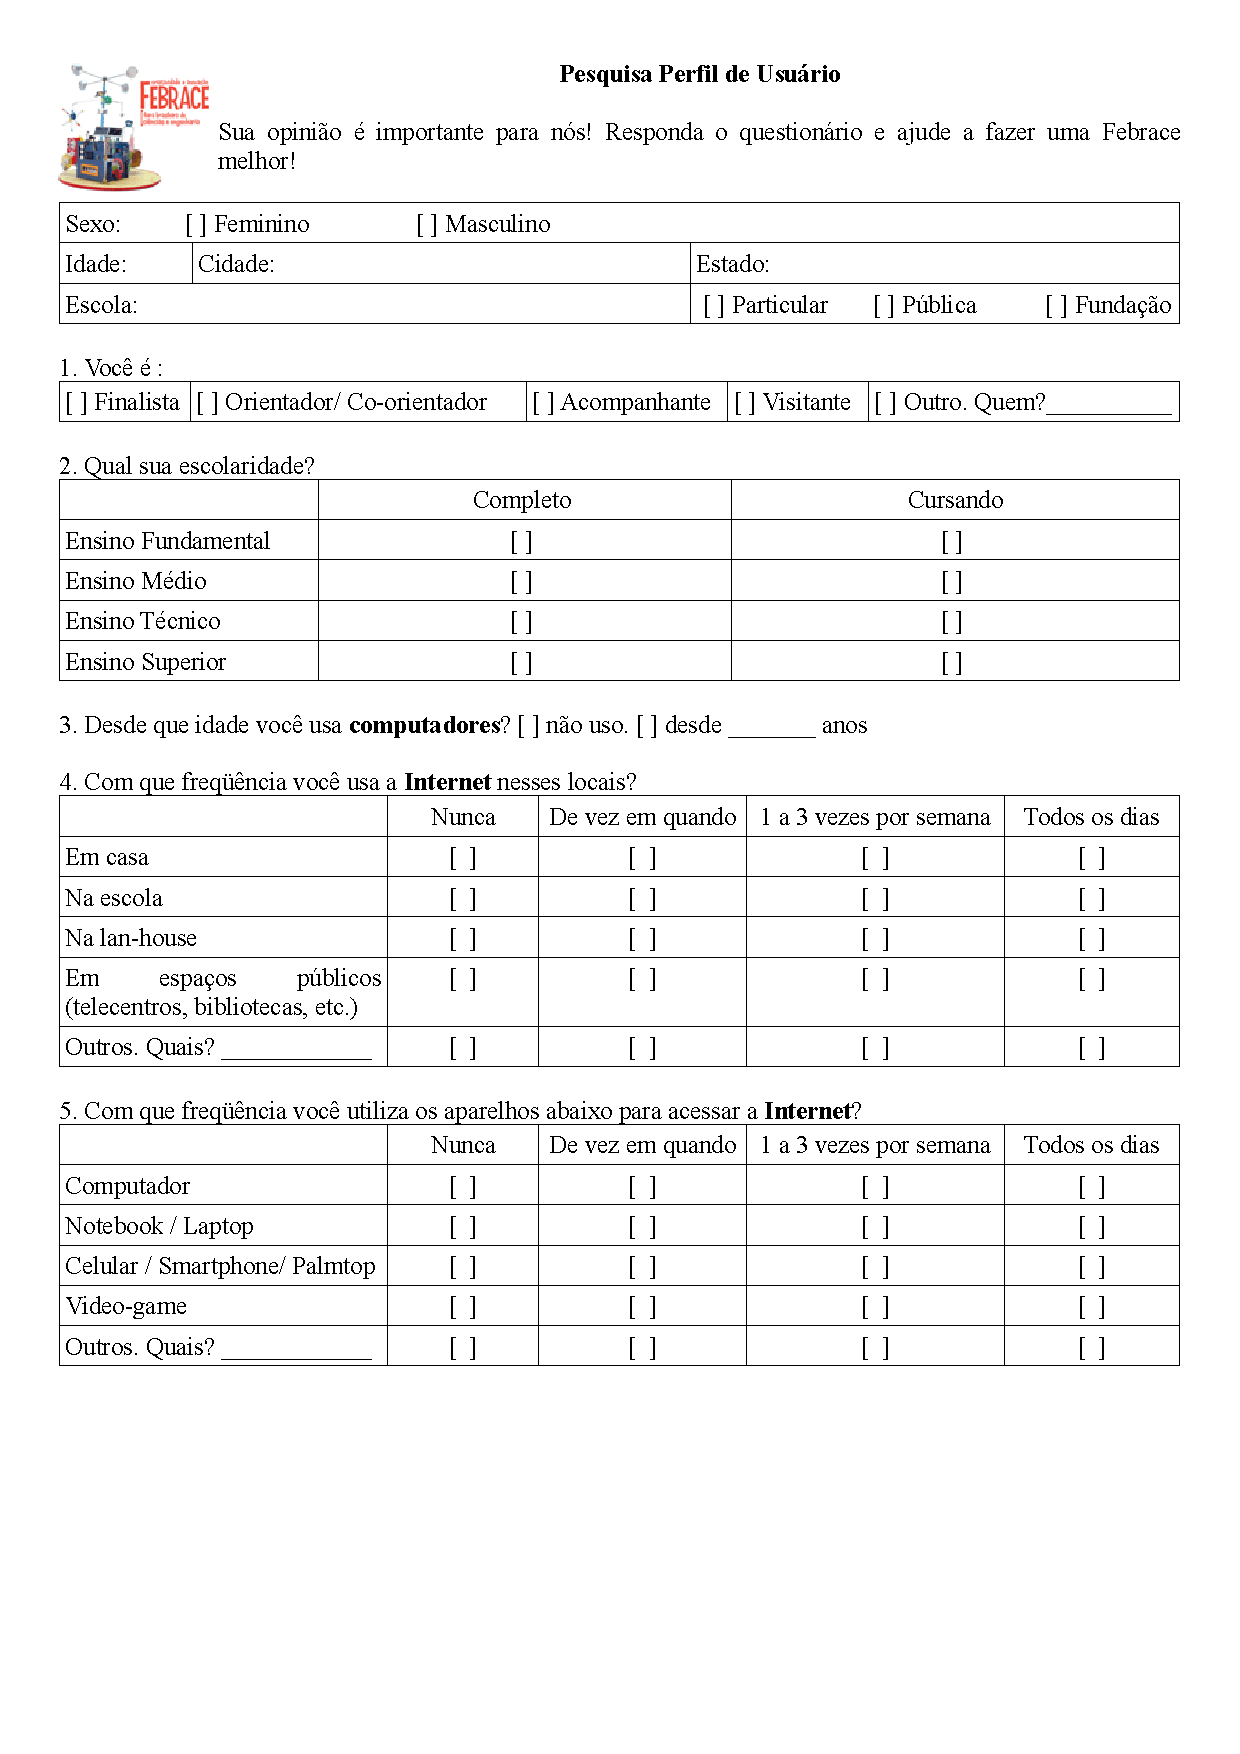
\includepdf[pages={1-2}]{questionario}

\end{document}
